\documentclass{article}

\usepackage[utf8]{inputenc}
%\usepackage[spanish]{babel}
\usepackage[spanish,es-tabla]{babel}
% Set page size and margins
% Replace `letterpaper' with `a4paper' for UK/EU standard size
% \usepackage[letterpaper,top=2cm,bottom=2cm,left=3cm,right=3cm,marginparwidth=1.75cm]{geometry}
\usepackage[a4paper,margin=1in]{geometry}
% Useful packages
\usepackage{amsmath}
\usepackage{graphicx}
\usepackage[colorlinks=true, allcolors=blue]{hyperref}

\usepackage{subcaption}
\usepackage{amssymb}
\usepackage{mathtools}
\usepackage[table,xcdraw]{xcolor}
\usepackage[backend=bibtex]{biblatex}
\usepackage{csquotes}
\usepackage{float}

\addbibresource{bibliografia.bib}


\begin{document}

% agregamos la caratula
\begin{titlepage}

\begin{center}
    
\includegraphics[width=5cm]{img/unc_logo.png} \hspace{2cm}
    
\includegraphics[width=5cm]{img/fcefyn_logo.jpg}
    \\[1cm]
    \vspace{5pt}
    \LARGE Universidad Nacional de Córdoba\\[0.6cm] 
    \large Facultad de Ciencias Exactas, Físicas y Naturales 
    \\[4cm] 
    \large Laboratorio N° 1
    \\[0.8cm]
    \large “AO Real: Errores”
    \\[0.2cm]
    \vspace{60pt}
    \begin{table}[!h]
    
    \centering
    \begin{tabular}{ll}
    \multicolumn{1}{c}{Integrantes} \\
    Britez, Fabio\\
    Corvalán, Abel \\
    Rodriguez, Facundo Nicolas 
    \end{tabular}
    \end{table}
    \vspace{20pt}
    \begin{table}[!h]
    \centering
    
    \begin{tabular}{ll}
    \multicolumn{1}{c}{Docente:} & Ing. Pablo Ferreyra
    \end{tabular}
    \end{table}
    \vfill
    Córdoba, República Argentina\\
    \today
\end{center}

\end{titlepage}
\newpage

% agregamos el indice
\tableofcontents
\newpage



\section{Introducción}



%Analisis1
\section{Circuito N° 1}



\subsection{Esquematico y datos}

Se realiza el análisis teórico del circuito que se muestra en la siguiente figura. 
 

\begin{figure}[h!]
    \centering
    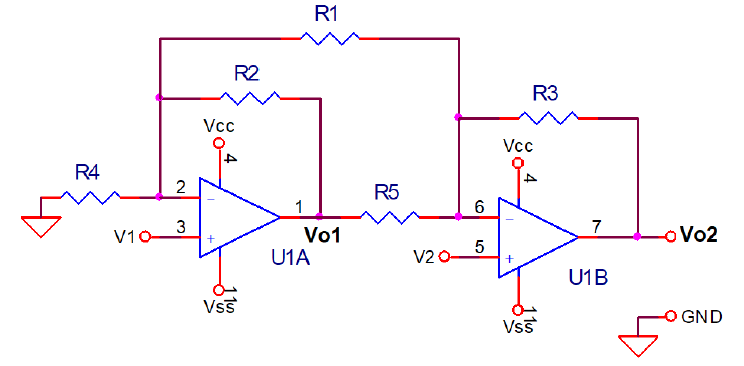
\includegraphics[width=0.80\linewidth]{Secciones/Circuito1/esquematico.png}
    \caption{Esquematico del circuito N° 1}
    \label{fig:esquematico}
\end{figure}

Datos:

\begin{itemize}
  \item Amplificador operacional: LM324
  \item $V_{cc} = 10 \, \text{[V]}$
  \item $V_{ss} = -10 \, \text{[V]}$
  \item $R_1 = R_2 = R_3 = R_4 = R_5 = R$
\end{itemize}

\subsection{Análisis teorico}
Para facilitar el analisis del circuito, consideramos AO ideal, dividimos en 2 casos y luego aplicaremos el teorema de la superposición.

\vspace{1em}

\textbf{Caso 1:} Pasivamos la fuente $V_2$, quedando asi: $V_1 \neq 0 $ y $V_2 = 0$ .

\vspace{1em}

Primero calculamos la ganancia $\frac{V_{O1}}{V_1}$ de la primer etapa. Para esto tengamos en cuenta que $R_1$ y $R_4$ quedan en paralelo. 

\vspace{1em}

\[{R_p = {(R_1 // R_4)} = \frac{R_1 \cdot R_4}{R_1 + R_4}}\]

Luego tenemos que: 

\[I_{R_2} = I_{R_p}\]

\[\frac{V_{01} - V_1}{R_2}
      = \frac{V_1 - 0}{R_p}\]

Si distribuimos y reagrupamos terminos.

\[\frac{V_{01}}{R_2} = (\frac{1}{R_p}+\frac{1}{R_2}) \cdot {V_1}\]
      
\[{V_{01}} = (\frac{R_2}{R_p}+{1}) \cdot {V_1}\]

Por lo tanto la primera etapa queda como un no inversor:


\begin{equation}\label{eq:primera_etapa} 
\frac{V_{01}}{V_1} = \frac{R_2}{R_p}+{1}
\end{equation}

      
Ahora calculamos la ganancia $\frac{V_{02}}{V_{01}}$ de la se la segunda etapa:

\[I_{R_3} = I_{R_5}\]


\[\frac{V_{02} - 0 }{R_3} = \frac{0 - V_{01}}{R_5}\]


Despejamos y obtenemos la ganancia de la segunda etapa con respecto a la primera:

\[V_{02} = -(\frac{R_3}{R_5}) \cdot {V_{01}}\]   


\begin{equation}\label{eq:segunda_etapa} 
\frac{V_{02}}{V_{01}} = -\frac{R_3}{R_5}
\end{equation}

Por lo tanto la ganancia para el Caso 1, reemplazando \eqref{eq:primera_etapa} en \eqref{eq:segunda_etapa} tenemos:

\[ A_{V1} = \frac{V_{02}}{V_{01}} \cdot \frac{V_{01}}{V_1} = -\frac{R_3}{R_5} \cdot (\frac{R_2}{R_p}+{1})  \]

\vspace{1em}

\textbf{Caso 2:} Pasivamos la fuente $V_1$, quedando asi: $V_1 = 0$ y $V_2 \neq 0$

\vspace{1em}

Aplicamos la ley de las corrientes en los nodos en la primer etapa:


\[I_{R2} + I_{R1} = 0 \]


\[\frac{V_{01}}{R_2} = -\frac{V_2}{R_1}\]


\[{V_{01}} = -(\frac{R_2}{R_1}) \cdot {V_2}\]

Considerando que lo siguiente:

\[{R_1}={R_2}={R_3}={R_4}={R_5}
      = {R}\]
Entonces, se tiene:
 
 
 \[{V_{01}} = -{V_2}\]
Analizando la segunda etapa se tiene:

\[\frac{V_o-V_2}{R_3}
      = \frac{V_2-V_x}{R_5}+\frac{V_2}{R_1}\]
\[\frac{V_o}{R_3}
      = (\frac{1}{R_5}+\frac{1}{R_1}+\frac{1}{R_1})*{V_2}-\frac{V_x}{R_5}\]

Por la condición (1) se tiene
      \[{V_o}=3*{V_2}+{V_2}\]
      \[{V_o}=4*{V_2}\]
      
\subsection{Análisis de modo diferencial }

En el análisis de modo diferencial se considera
 \[V_2 \neq V_1\]
\[{v_d}
      = {v_2-v_1}\]
      
\subsection{Análisis de modo común}

En el análisis de modo común:

\[{v_c}
      = \frac{v_1+v_2}{2}\]

\subsection{Simulación}

Se realiza la simulación del circuito en el software LTSpice:

\begin{figure}[h!]
    \centering
    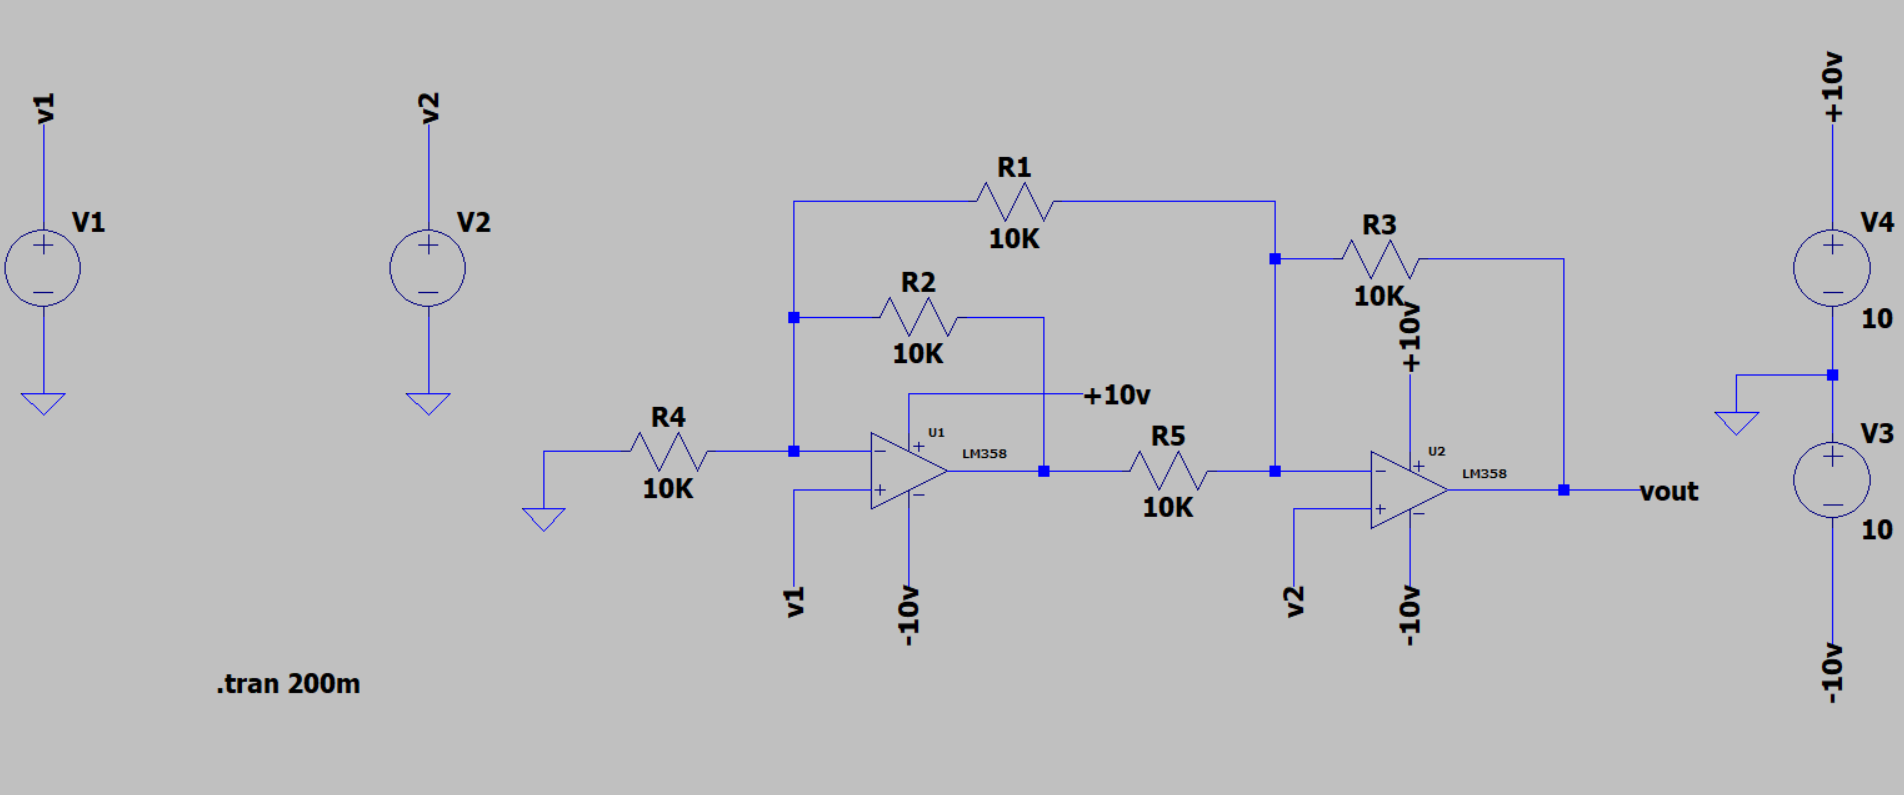
\includegraphics[width=1\linewidth]{Secciones/Circuito1/circuito1_simulacion.png}
    \caption{Señal de salida para modo diferencial - Circuito 1}
    \label{fig:enter-label}
\end{figure}

con señal de entrada en modo diferencial:

\begin{figure}[h!]
    \centering
    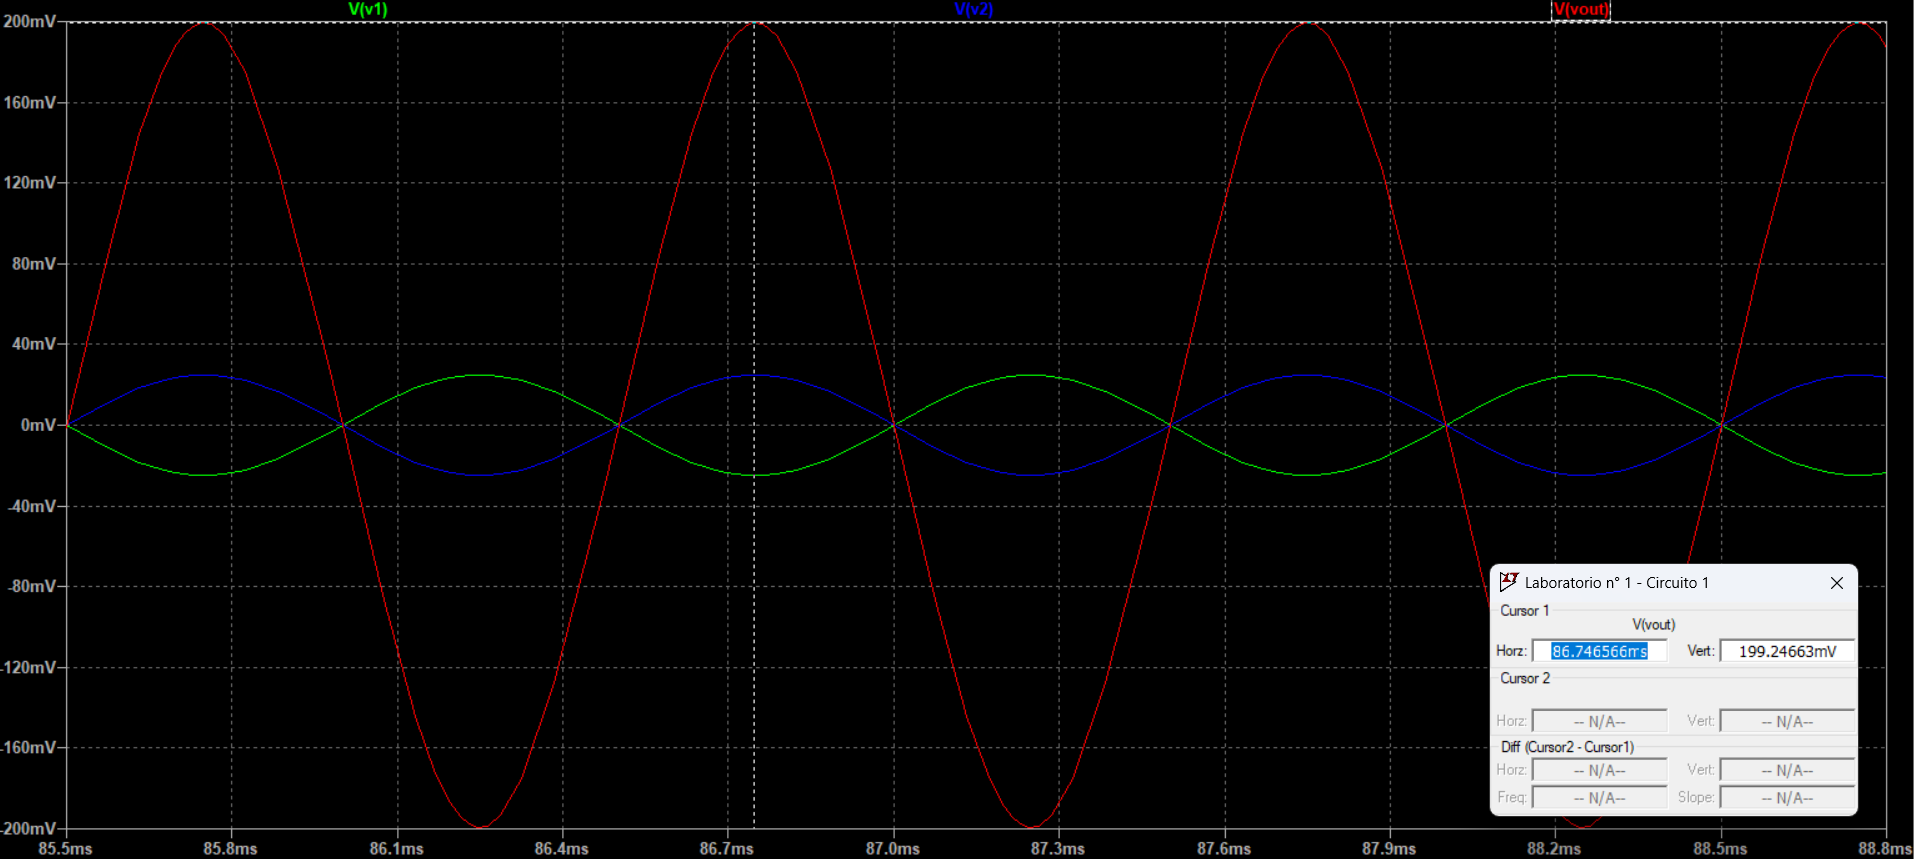
\includegraphics[width=1\linewidth]{Secciones/Circuito1/circuito1_diferencial.png}
    
    \caption{Señal de salida para modo diferencial - Circuito 1}
    \label{fig:enter-label}
\end{figure}

Se realizan las siguientes mediciones:
    
\begin{table}[ht]
    \centering


    \begin{tabular}{|p{0.3\linewidth}  |p{0.6\linewidth}  |p{0.6\linewidth}  |p{0.6\linewidth}  |p{0.6\linewidth}|} \hline 
      Condiciones de medición & \[V1\neq0 \space y \space V2=0 \] & \[V1=0 \space y \space   V2\neq0 \] & \[V1=V2\neq0, \Delta\varphi=0\]
      & \[V1=V2\neq0, \Delta\varphi\neq0\] \\ \hline
      Vo [mV] & 25& 25& & Next
     \\ \hline\end{tabular}
    
    
\end{table}

Se presenta el diagrama de Bode de nuestro circuito.
\newpage

%Analisis2
\section{Circuito N° 1}



\subsection{Esquematico y datos}

Se realiza el análisis teórico del circuito que se muestra en la siguiente figura. 
 

\begin{figure}[h!]
    \centering
    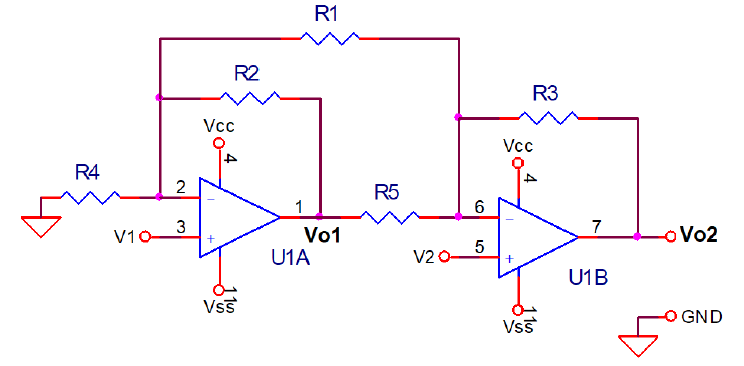
\includegraphics[width=0.80\linewidth]{Secciones/Circuito1/esquematico.png}
    \caption{Esquematico del circuito N° 1}
    \label{fig:esquematico}
\end{figure}

Datos:

\begin{itemize}
  \item Amplificador operacional: LM324
  \item $V_{cc} = 10 \, \text{[V]}$
  \item $V_{ss} = -10 \, \text{[V]}$
  \item $R_1 = R_2 = R_3 = R_4 = R_5 = R$
\end{itemize}

\subsection{Análisis teorico}
Para facilitar el analisis del circuito, consideramos AO ideal, dividimos en 2 casos y luego aplicaremos el teorema de la superposición.

\vspace{1em}

\textbf{Caso 1:} Pasivamos la fuente $V_2$, quedando asi: $V_1 \neq 0 $ y $V_2 = 0$ .

\vspace{1em}

Primero calculamos la ganancia $\frac{V_{O1}}{V_1}$ de la primer etapa. Para esto tengamos en cuenta que $R_1$ y $R_4$ quedan en paralelo. 

\vspace{1em}

\[{R_p = {(R_1 // R_4)} = \frac{R_1 \cdot R_4}{R_1 + R_4}}\]

Luego tenemos que: 

\[I_{R_2} = I_{R_p}\]

\[\frac{V_{01} - V_1}{R_2}
      = \frac{V_1 - 0}{R_p}\]

Si distribuimos y reagrupamos terminos.

\[\frac{V_{01}}{R_2} = (\frac{1}{R_p}+\frac{1}{R_2}) \cdot {V_1}\]
      
\[{V_{01}} = (\frac{R_2}{R_p}+{1}) \cdot {V_1}\]

Por lo tanto la primera etapa queda como un no inversor:


\begin{equation}\label{eq:primera_etapa} 
\frac{V_{01}}{V_1} = \frac{R_2}{R_p}+{1}
\end{equation}

      
Ahora calculamos la ganancia $\frac{V_{02}}{V_{01}}$ de la se la segunda etapa:

\[I_{R_3} = I_{R_5}\]


\[\frac{V_{02} - 0 }{R_3} = \frac{0 - V_{01}}{R_5}\]


Despejamos y obtenemos la ganancia de la segunda etapa con respecto a la primera:

\[V_{02} = -(\frac{R_3}{R_5}) \cdot {V_{01}}\]   


\begin{equation}\label{eq:segunda_etapa} 
\frac{V_{02}}{V_{01}} = -\frac{R_3}{R_5}
\end{equation}

Por lo tanto la ganancia para el Caso 1, reemplazando \eqref{eq:primera_etapa} en \eqref{eq:segunda_etapa} tenemos:

\[ A_{V1} = \frac{V_{02}}{V_{01}} \cdot \frac{V_{01}}{V_1} = -\frac{R_3}{R_5} \cdot (\frac{R_2}{R_p}+{1})  \]

\vspace{1em}

\textbf{Caso 2:} Pasivamos la fuente $V_1$, quedando asi: $V_1 = 0$ y $V_2 \neq 0$

\vspace{1em}

Aplicamos la ley de las corrientes en los nodos en la primer etapa:


\[I_{R2} + I_{R1} = 0 \]


\[\frac{V_{01}}{R_2} = -\frac{V_2}{R_1}\]


\[{V_{01}} = -(\frac{R_2}{R_1}) \cdot {V_2}\]

Considerando que lo siguiente:

\[{R_1}={R_2}={R_3}={R_4}={R_5}
      = {R}\]
Entonces, se tiene:
 
 
 \[{V_{01}} = -{V_2}\]
Analizando la segunda etapa se tiene:

\[\frac{V_o-V_2}{R_3}
      = \frac{V_2-V_x}{R_5}+\frac{V_2}{R_1}\]
\[\frac{V_o}{R_3}
      = (\frac{1}{R_5}+\frac{1}{R_1}+\frac{1}{R_1})*{V_2}-\frac{V_x}{R_5}\]

Por la condición (1) se tiene
      \[{V_o}=3*{V_2}+{V_2}\]
      \[{V_o}=4*{V_2}\]
      
\subsection{Análisis de modo diferencial }

En el análisis de modo diferencial se considera
 \[V_2 \neq V_1\]
\[{v_d}
      = {v_2-v_1}\]
      
\subsection{Análisis de modo común}

En el análisis de modo común:

\[{v_c}
      = \frac{v_1+v_2}{2}\]

\subsection{Simulación}

Se realiza la simulación del circuito en el software LTSpice:

\begin{figure}[h!]
    \centering
    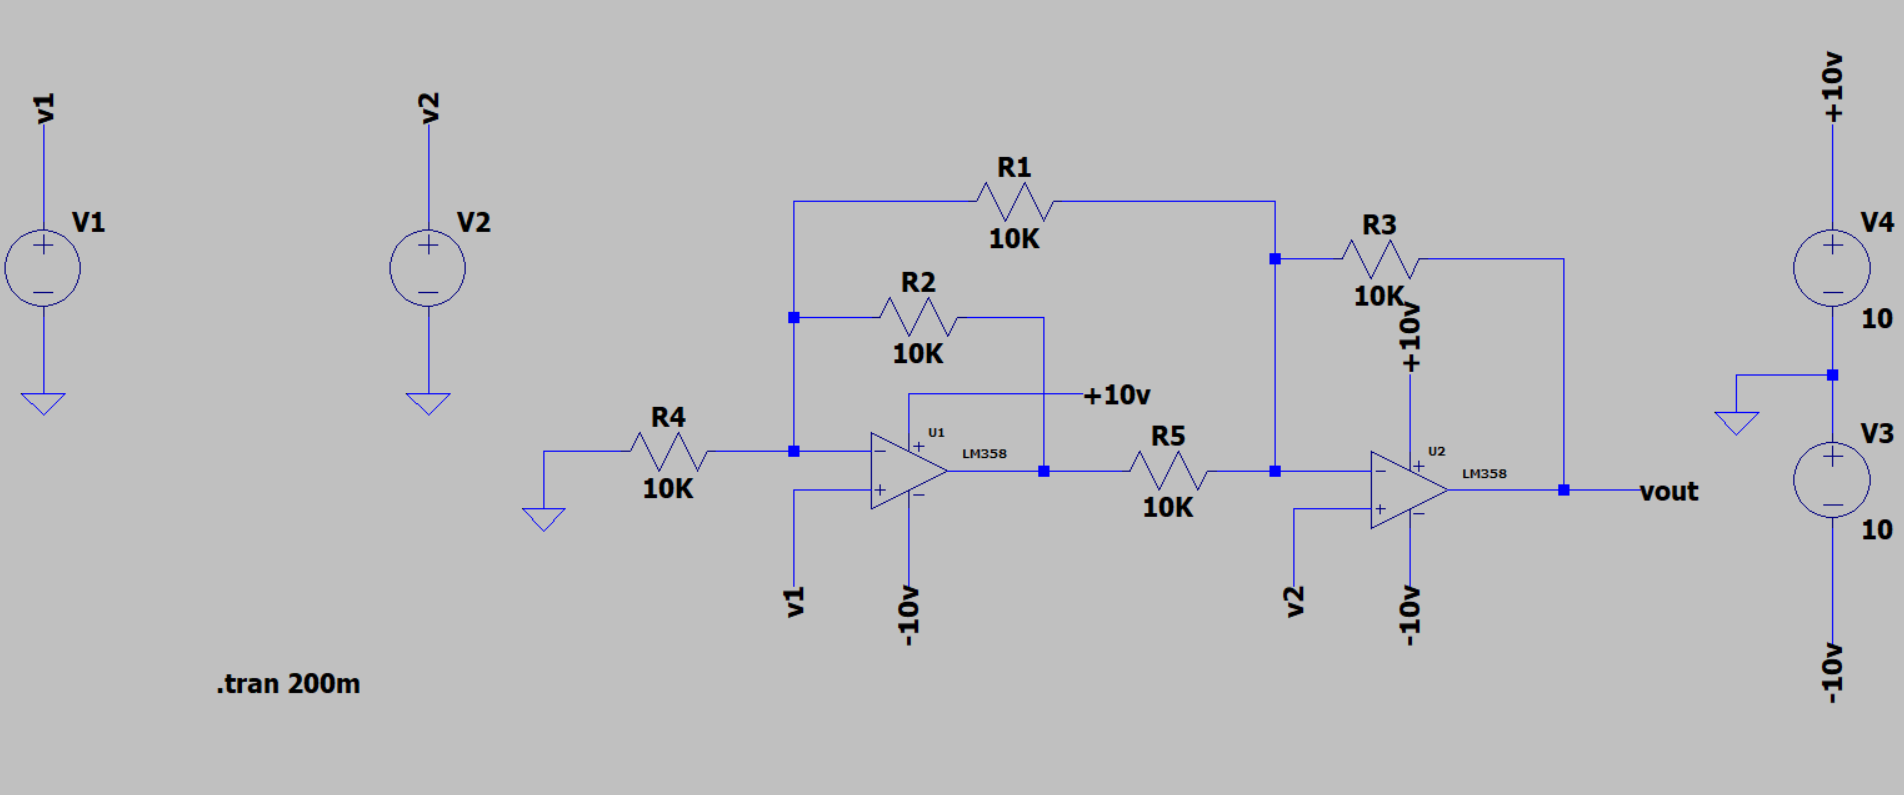
\includegraphics[width=1\linewidth]{Secciones/Circuito1/circuito1_simulacion.png}
    \caption{Señal de salida para modo diferencial - Circuito 1}
    \label{fig:enter-label}
\end{figure}

con señal de entrada en modo diferencial:

\begin{figure}[h!]
    \centering
    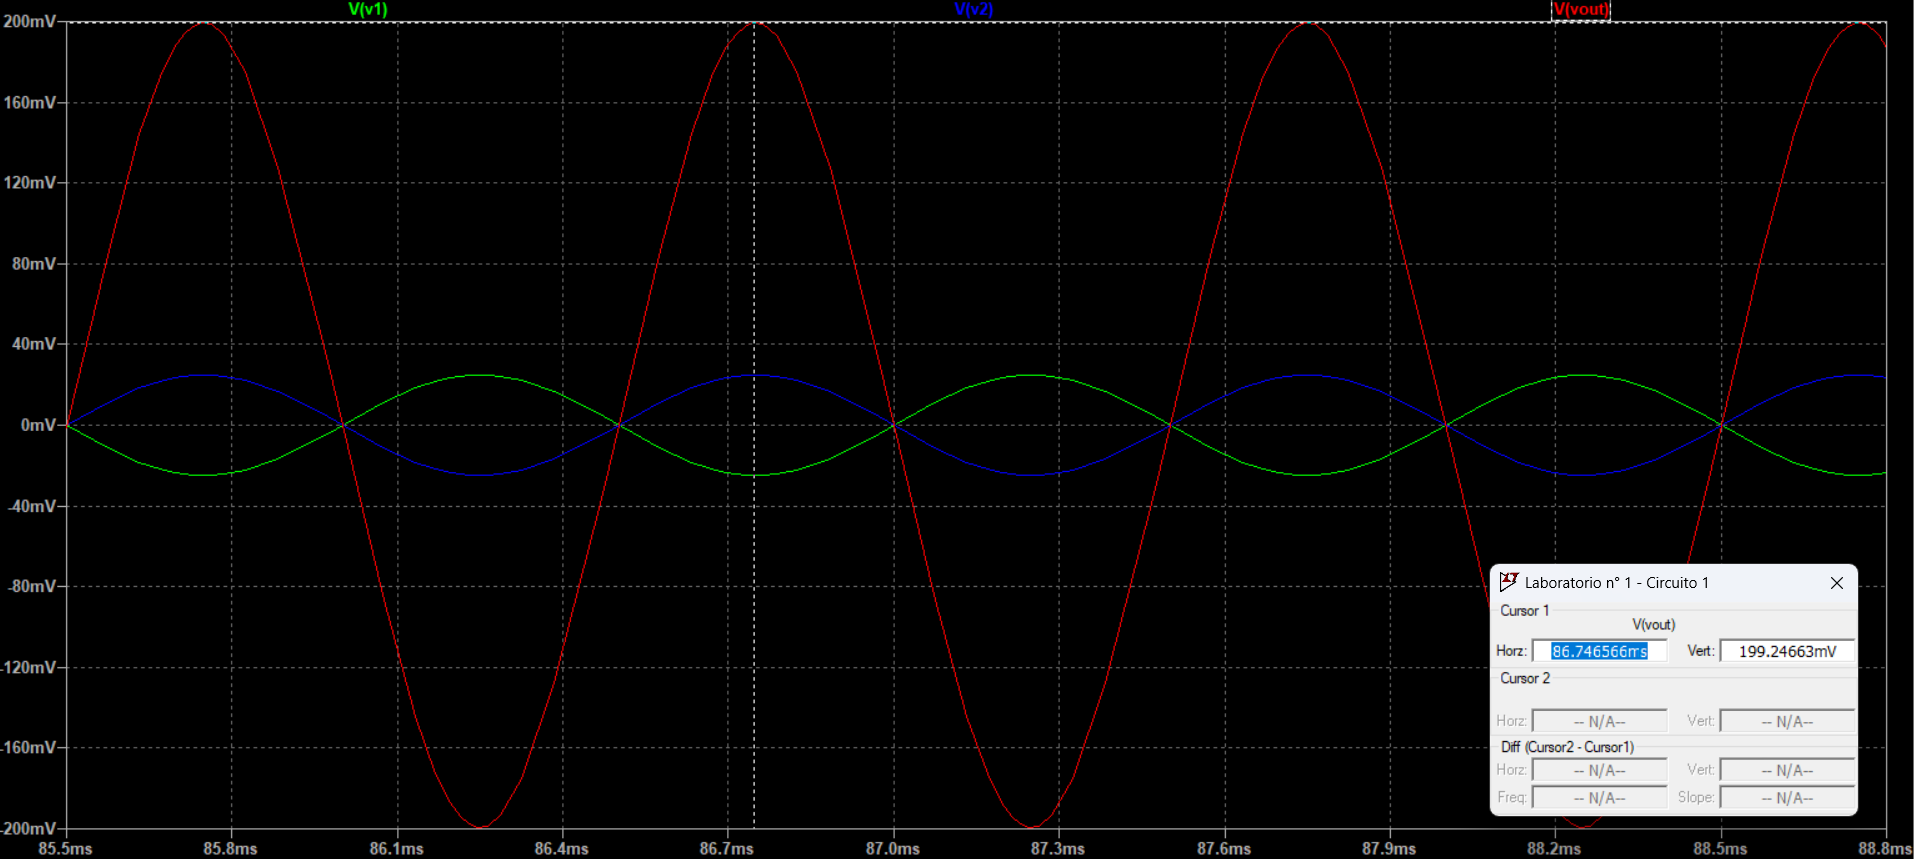
\includegraphics[width=1\linewidth]{Secciones/Circuito1/circuito1_diferencial.png}
    
    \caption{Señal de salida para modo diferencial - Circuito 1}
    \label{fig:enter-label}
\end{figure}

Se realizan las siguientes mediciones:
    
\begin{table}[ht]
    \centering


    \begin{tabular}{|p{0.3\linewidth}  |p{0.6\linewidth}  |p{0.6\linewidth}  |p{0.6\linewidth}  |p{0.6\linewidth}|} \hline 
      Condiciones de medición & \[V1\neq0 \space y \space V2=0 \] & \[V1=0 \space y \space   V2\neq0 \] & \[V1=V2\neq0, \Delta\varphi=0\]
      & \[V1=V2\neq0, \Delta\varphi\neq0\] \\ \hline
      Vo [mV] & 25& 25& & Next
     \\ \hline\end{tabular}
    
    
\end{table}

Se presenta el diagrama de Bode de nuestro circuito.
\newpage

 \section{Circuito N° 1}



\subsection{Esquematico y datos}

Se realiza el análisis teórico del circuito que se muestra en la siguiente figura. 
 

\begin{figure}[h!]
    \centering
    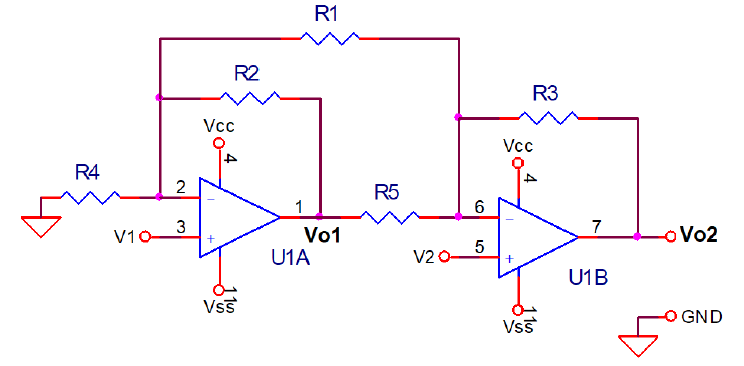
\includegraphics[width=0.80\linewidth]{Secciones/Circuito1/esquematico.png}
    \caption{Esquematico del circuito N° 1}
    \label{fig:esquematico}
\end{figure}

Datos:

\begin{itemize}
  \item Amplificador operacional: LM324
  \item $V_{cc} = 10 \, \text{[V]}$
  \item $V_{ss} = -10 \, \text{[V]}$
  \item $R_1 = R_2 = R_3 = R_4 = R_5 = R$
\end{itemize}

\subsection{Análisis teorico}
Para facilitar el analisis del circuito, consideramos AO ideal, dividimos en 2 casos y luego aplicaremos el teorema de la superposición.

\vspace{1em}

\textbf{Caso 1:} Pasivamos la fuente $V_2$, quedando asi: $V_1 \neq 0 $ y $V_2 = 0$ .

\vspace{1em}

Primero calculamos la ganancia $\frac{V_{O1}}{V_1}$ de la primer etapa. Para esto tengamos en cuenta que $R_1$ y $R_4$ quedan en paralelo. 

\vspace{1em}

\[{R_p = {(R_1 // R_4)} = \frac{R_1 \cdot R_4}{R_1 + R_4}}\]

Luego tenemos que: 

\[I_{R_2} = I_{R_p}\]

\[\frac{V_{01} - V_1}{R_2}
      = \frac{V_1 - 0}{R_p}\]

Si distribuimos y reagrupamos terminos.

\[\frac{V_{01}}{R_2} = (\frac{1}{R_p}+\frac{1}{R_2}) \cdot {V_1}\]
      
\[{V_{01}} = (\frac{R_2}{R_p}+{1}) \cdot {V_1}\]

Por lo tanto la primera etapa queda como un no inversor:


\begin{equation}\label{eq:primera_etapa} 
\frac{V_{01}}{V_1} = \frac{R_2}{R_p}+{1}
\end{equation}

      
Ahora calculamos la ganancia $\frac{V_{02}}{V_{01}}$ de la se la segunda etapa:

\[I_{R_3} = I_{R_5}\]


\[\frac{V_{02} - 0 }{R_3} = \frac{0 - V_{01}}{R_5}\]


Despejamos y obtenemos la ganancia de la segunda etapa con respecto a la primera:

\[V_{02} = -(\frac{R_3}{R_5}) \cdot {V_{01}}\]   


\begin{equation}\label{eq:segunda_etapa} 
\frac{V_{02}}{V_{01}} = -\frac{R_3}{R_5}
\end{equation}

Por lo tanto la ganancia para el Caso 1, reemplazando \eqref{eq:primera_etapa} en \eqref{eq:segunda_etapa} tenemos:

\[ A_{V1} = \frac{V_{02}}{V_{01}} \cdot \frac{V_{01}}{V_1} = -\frac{R_3}{R_5} \cdot (\frac{R_2}{R_p}+{1})  \]

\vspace{1em}

\textbf{Caso 2:} Pasivamos la fuente $V_1$, quedando asi: $V_1 = 0$ y $V_2 \neq 0$

\vspace{1em}

Aplicamos la ley de las corrientes en los nodos en la primer etapa:


\[I_{R2} + I_{R1} = 0 \]


\[\frac{V_{01}}{R_2} = -\frac{V_2}{R_1}\]


\[{V_{01}} = -(\frac{R_2}{R_1}) \cdot {V_2}\]

Considerando que lo siguiente:

\[{R_1}={R_2}={R_3}={R_4}={R_5}
      = {R}\]
Entonces, se tiene:
 
 
 \[{V_{01}} = -{V_2}\]
Analizando la segunda etapa se tiene:

\[\frac{V_o-V_2}{R_3}
      = \frac{V_2-V_x}{R_5}+\frac{V_2}{R_1}\]
\[\frac{V_o}{R_3}
      = (\frac{1}{R_5}+\frac{1}{R_1}+\frac{1}{R_1})*{V_2}-\frac{V_x}{R_5}\]

Por la condición (1) se tiene
      \[{V_o}=3*{V_2}+{V_2}\]
      \[{V_o}=4*{V_2}\]
      
\subsection{Análisis de modo diferencial }

En el análisis de modo diferencial se considera
 \[V_2 \neq V_1\]
\[{v_d}
      = {v_2-v_1}\]
      
\subsection{Análisis de modo común}

En el análisis de modo común:

\[{v_c}
      = \frac{v_1+v_2}{2}\]

\subsection{Simulación}

Se realiza la simulación del circuito en el software LTSpice:

\begin{figure}[h!]
    \centering
    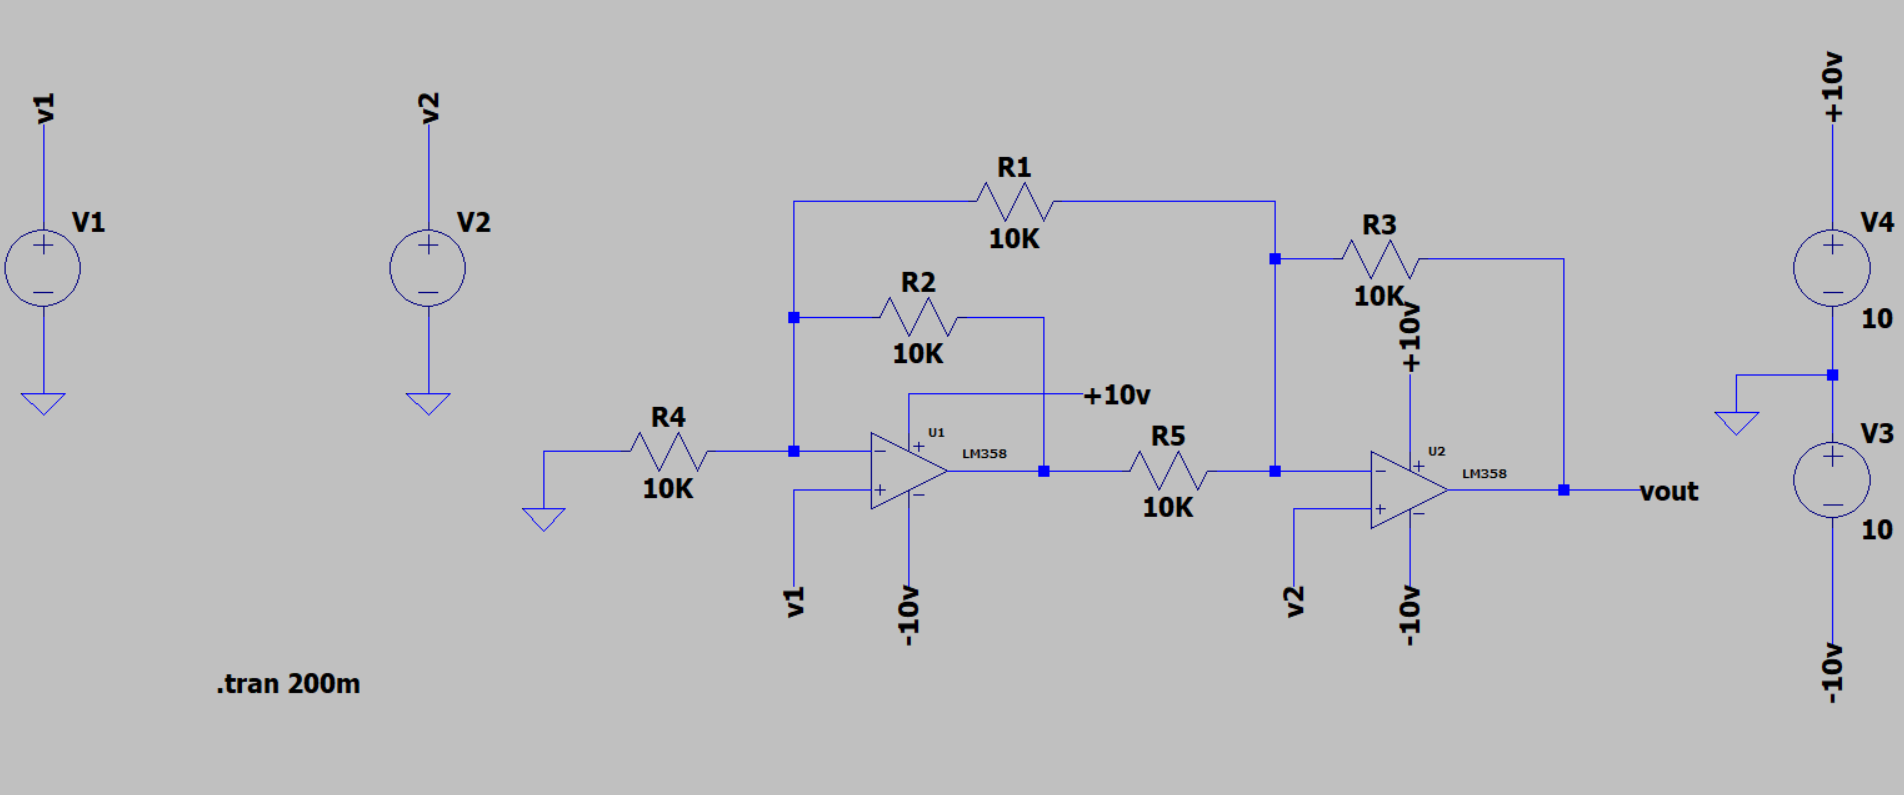
\includegraphics[width=1\linewidth]{Secciones/Circuito1/circuito1_simulacion.png}
    \caption{Señal de salida para modo diferencial - Circuito 1}
    \label{fig:enter-label}
\end{figure}

con señal de entrada en modo diferencial:

\begin{figure}[h!]
    \centering
    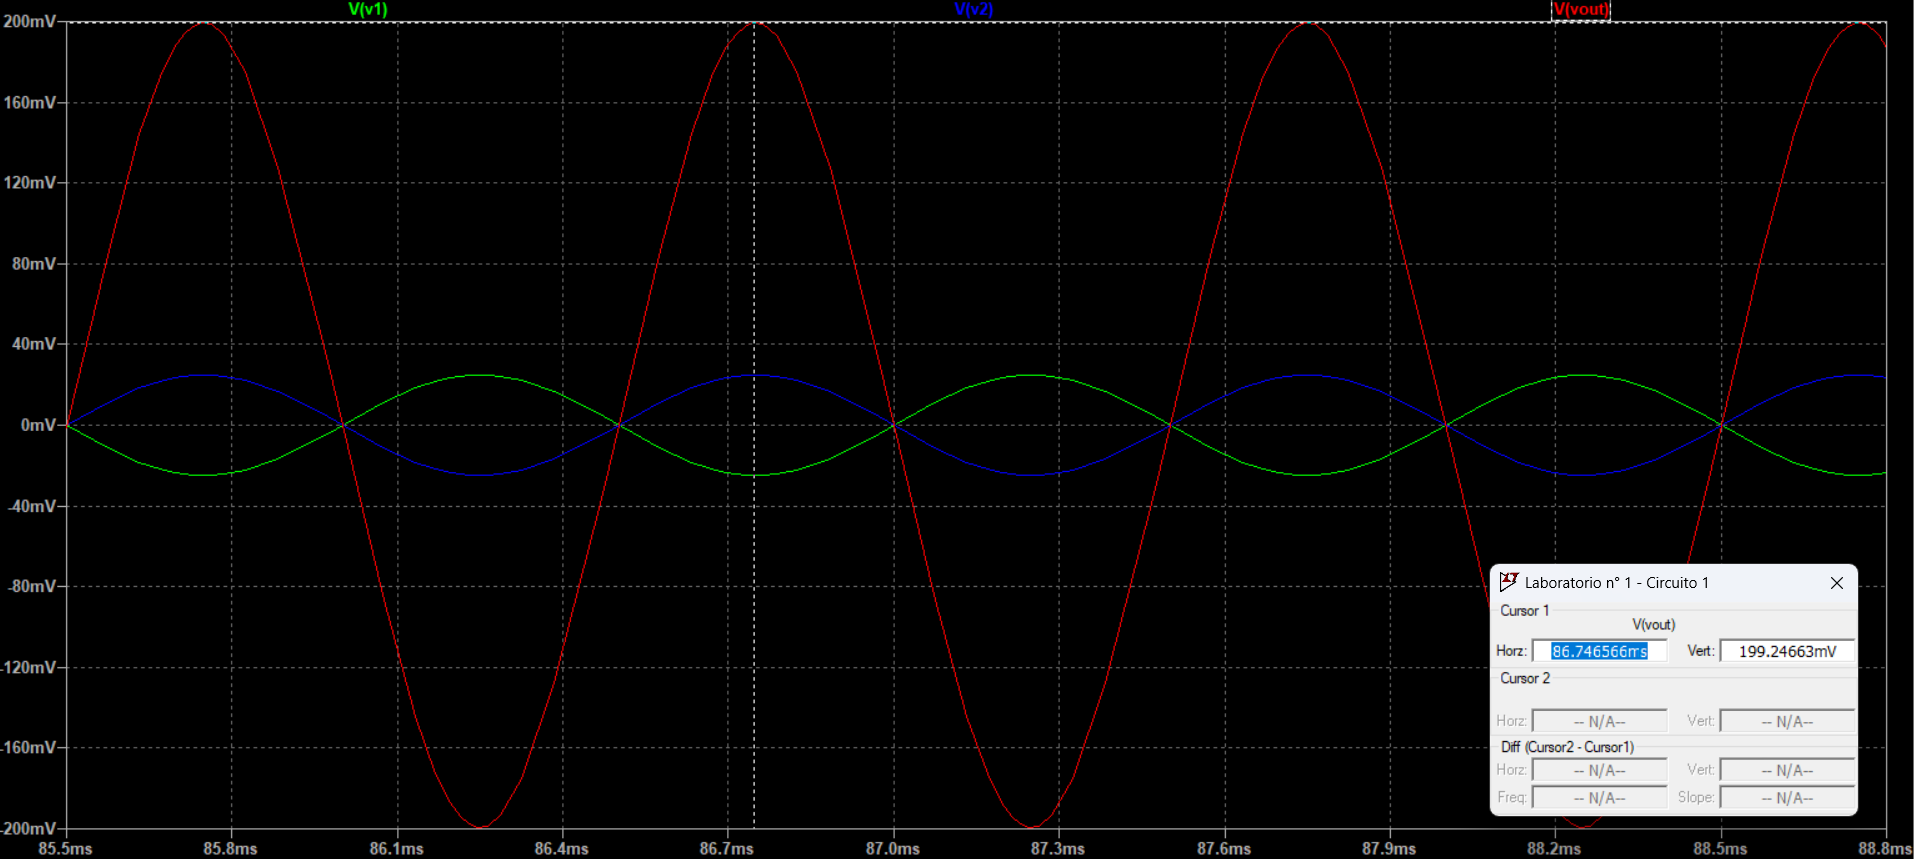
\includegraphics[width=1\linewidth]{Secciones/Circuito1/circuito1_diferencial.png}
    
    \caption{Señal de salida para modo diferencial - Circuito 1}
    \label{fig:enter-label}
\end{figure}

Se realizan las siguientes mediciones:
    
\begin{table}[ht]
    \centering


    \begin{tabular}{|p{0.3\linewidth}  |p{0.6\linewidth}  |p{0.6\linewidth}  |p{0.6\linewidth}  |p{0.6\linewidth}|} \hline 
      Condiciones de medición & \[V1\neq0 \space y \space V2=0 \] & \[V1=0 \space y \space   V2\neq0 \] & \[V1=V2\neq0, \Delta\varphi=0\]
      & \[V1=V2\neq0, \Delta\varphi\neq0\] \\ \hline
      Vo [mV] & 25& 25& & Next
     \\ \hline\end{tabular}
    
    
\end{table}

Se presenta el diagrama de Bode de nuestro circuito.
\newpage

\section{Circuito N° 1}



\subsection{Esquematico y datos}

Se realiza el análisis teórico del circuito que se muestra en la siguiente figura. 
 

\begin{figure}[h!]
    \centering
    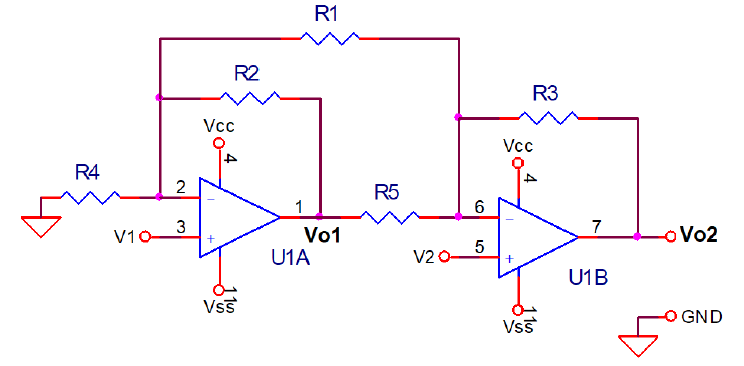
\includegraphics[width=0.80\linewidth]{Secciones/Circuito1/esquematico.png}
    \caption{Esquematico del circuito N° 1}
    \label{fig:esquematico}
\end{figure}

Datos:

\begin{itemize}
  \item Amplificador operacional: LM324
  \item $V_{cc} = 10 \, \text{[V]}$
  \item $V_{ss} = -10 \, \text{[V]}$
  \item $R_1 = R_2 = R_3 = R_4 = R_5 = R$
\end{itemize}

\subsection{Análisis teorico}
Para facilitar el analisis del circuito, consideramos AO ideal, dividimos en 2 casos y luego aplicaremos el teorema de la superposición.

\vspace{1em}

\textbf{Caso 1:} Pasivamos la fuente $V_2$, quedando asi: $V_1 \neq 0 $ y $V_2 = 0$ .

\vspace{1em}

Primero calculamos la ganancia $\frac{V_{O1}}{V_1}$ de la primer etapa. Para esto tengamos en cuenta que $R_1$ y $R_4$ quedan en paralelo. 

\vspace{1em}

\[{R_p = {(R_1 // R_4)} = \frac{R_1 \cdot R_4}{R_1 + R_4}}\]

Luego tenemos que: 

\[I_{R_2} = I_{R_p}\]

\[\frac{V_{01} - V_1}{R_2}
      = \frac{V_1 - 0}{R_p}\]

Si distribuimos y reagrupamos terminos.

\[\frac{V_{01}}{R_2} = (\frac{1}{R_p}+\frac{1}{R_2}) \cdot {V_1}\]
      
\[{V_{01}} = (\frac{R_2}{R_p}+{1}) \cdot {V_1}\]

Por lo tanto la primera etapa queda como un no inversor:


\begin{equation}\label{eq:primera_etapa} 
\frac{V_{01}}{V_1} = \frac{R_2}{R_p}+{1}
\end{equation}

      
Ahora calculamos la ganancia $\frac{V_{02}}{V_{01}}$ de la se la segunda etapa:

\[I_{R_3} = I_{R_5}\]


\[\frac{V_{02} - 0 }{R_3} = \frac{0 - V_{01}}{R_5}\]


Despejamos y obtenemos la ganancia de la segunda etapa con respecto a la primera:

\[V_{02} = -(\frac{R_3}{R_5}) \cdot {V_{01}}\]   


\begin{equation}\label{eq:segunda_etapa} 
\frac{V_{02}}{V_{01}} = -\frac{R_3}{R_5}
\end{equation}

Por lo tanto la ganancia para el Caso 1, reemplazando \eqref{eq:primera_etapa} en \eqref{eq:segunda_etapa} tenemos:

\[ A_{V1} = \frac{V_{02}}{V_{01}} \cdot \frac{V_{01}}{V_1} = -\frac{R_3}{R_5} \cdot (\frac{R_2}{R_p}+{1})  \]

\vspace{1em}

\textbf{Caso 2:} Pasivamos la fuente $V_1$, quedando asi: $V_1 = 0$ y $V_2 \neq 0$

\vspace{1em}

Aplicamos la ley de las corrientes en los nodos en la primer etapa:


\[I_{R2} + I_{R1} = 0 \]


\[\frac{V_{01}}{R_2} = -\frac{V_2}{R_1}\]


\[{V_{01}} = -(\frac{R_2}{R_1}) \cdot {V_2}\]

Considerando que lo siguiente:

\[{R_1}={R_2}={R_3}={R_4}={R_5}
      = {R}\]
Entonces, se tiene:
 
 
 \[{V_{01}} = -{V_2}\]
Analizando la segunda etapa se tiene:

\[\frac{V_o-V_2}{R_3}
      = \frac{V_2-V_x}{R_5}+\frac{V_2}{R_1}\]
\[\frac{V_o}{R_3}
      = (\frac{1}{R_5}+\frac{1}{R_1}+\frac{1}{R_1})*{V_2}-\frac{V_x}{R_5}\]

Por la condición (1) se tiene
      \[{V_o}=3*{V_2}+{V_2}\]
      \[{V_o}=4*{V_2}\]
      
\subsection{Análisis de modo diferencial }

En el análisis de modo diferencial se considera
 \[V_2 \neq V_1\]
\[{v_d}
      = {v_2-v_1}\]
      
\subsection{Análisis de modo común}

En el análisis de modo común:

\[{v_c}
      = \frac{v_1+v_2}{2}\]

\subsection{Simulación}

Se realiza la simulación del circuito en el software LTSpice:

\begin{figure}[h!]
    \centering
    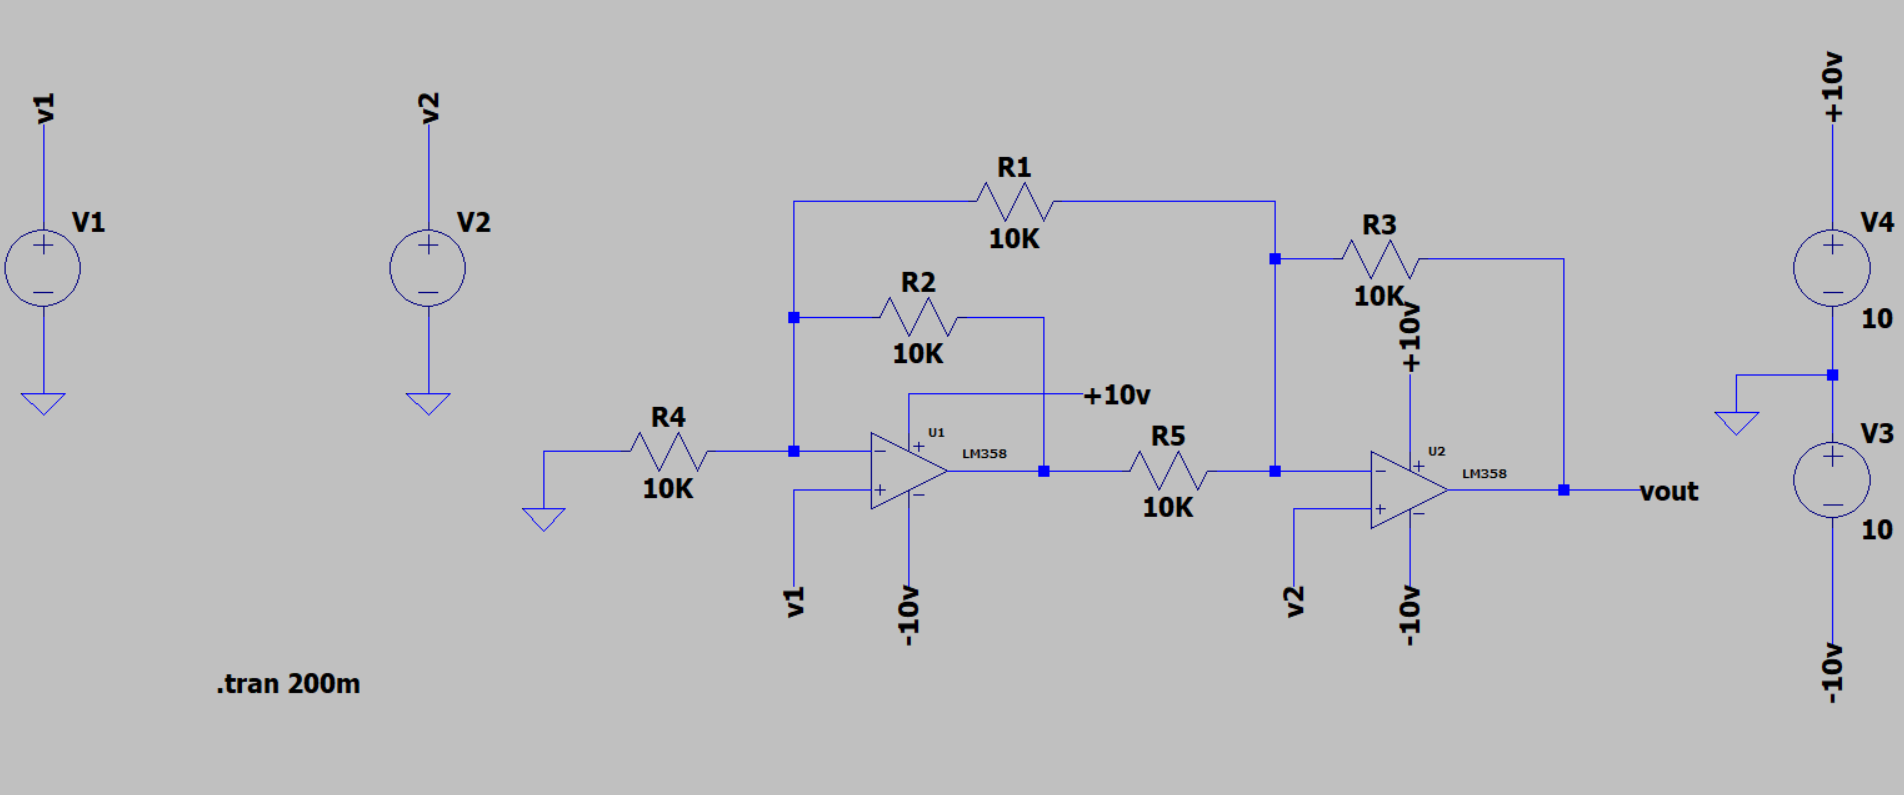
\includegraphics[width=1\linewidth]{Secciones/Circuito1/circuito1_simulacion.png}
    \caption{Señal de salida para modo diferencial - Circuito 1}
    \label{fig:enter-label}
\end{figure}

con señal de entrada en modo diferencial:

\begin{figure}[h!]
    \centering
    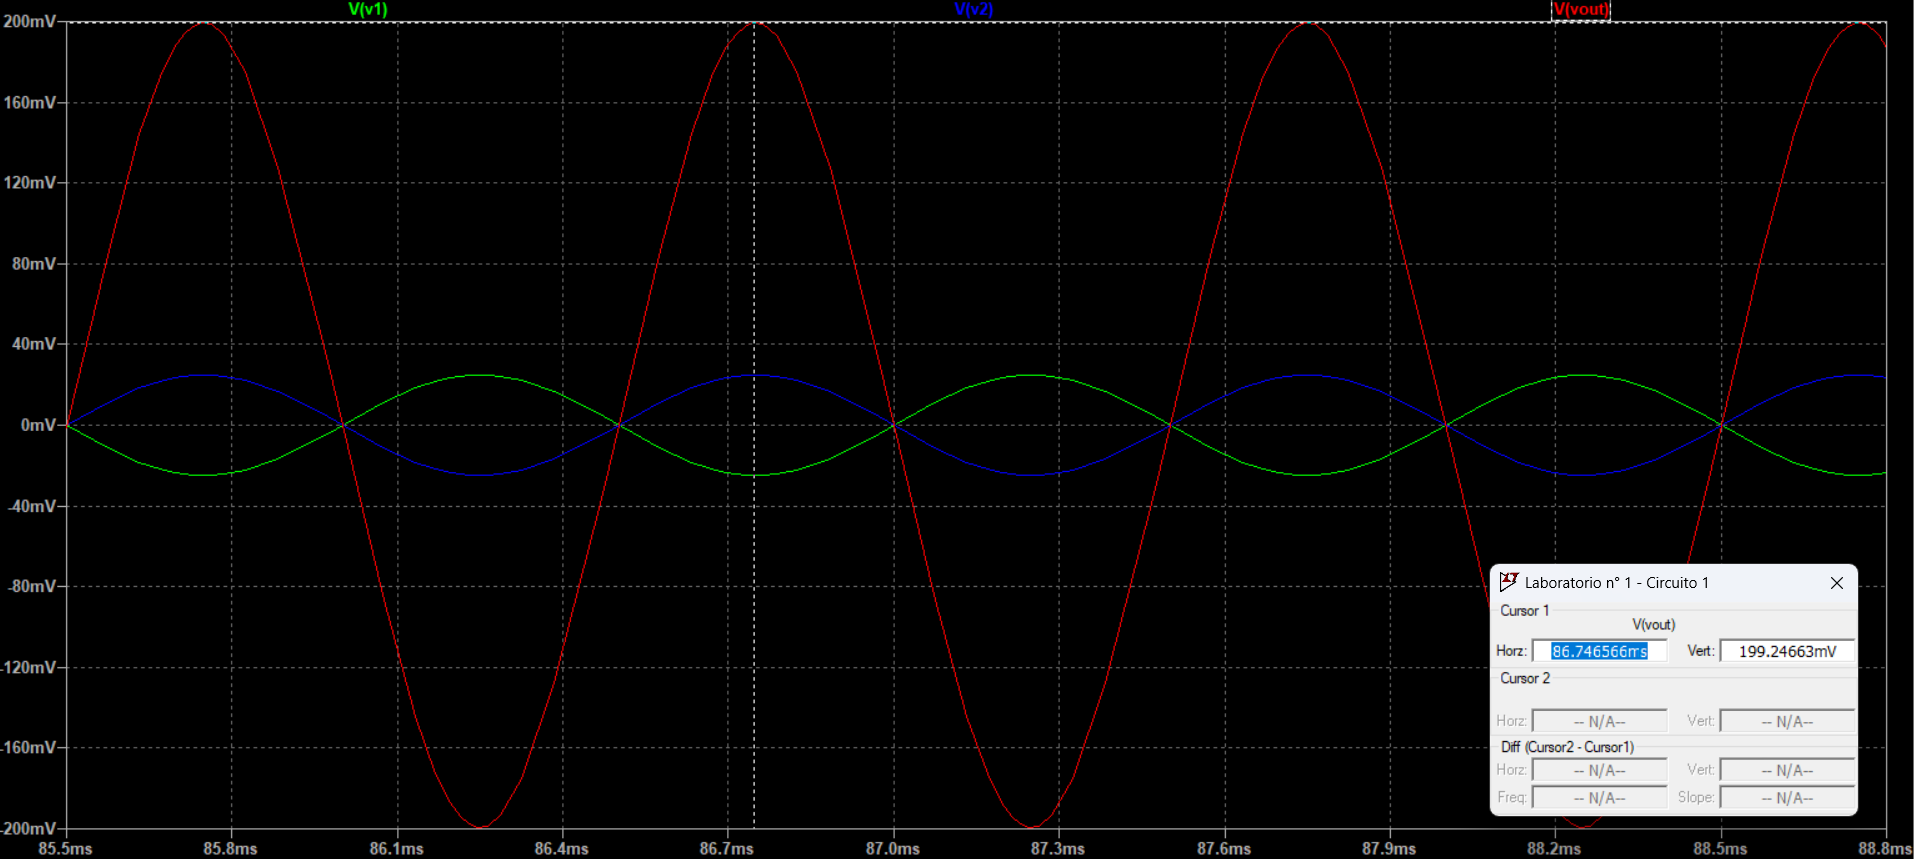
\includegraphics[width=1\linewidth]{Secciones/Circuito1/circuito1_diferencial.png}
    
    \caption{Señal de salida para modo diferencial - Circuito 1}
    \label{fig:enter-label}
\end{figure}

Se realizan las siguientes mediciones:
    
\begin{table}[ht]
    \centering


    \begin{tabular}{|p{0.3\linewidth}  |p{0.6\linewidth}  |p{0.6\linewidth}  |p{0.6\linewidth}  |p{0.6\linewidth}|} \hline 
      Condiciones de medición & \[V1\neq0 \space y \space V2=0 \] & \[V1=0 \space y \space   V2\neq0 \] & \[V1=V2\neq0, \Delta\varphi=0\]
      & \[V1=V2\neq0, \Delta\varphi\neq0\] \\ \hline
      Vo [mV] & 25& 25& & Next
     \\ \hline\end{tabular}
    
    
\end{table}

Se presenta el diagrama de Bode de nuestro circuito.
\newpage

\printbibliography

\end{document}
